%!TEX root = presentation.tex

\begin{frame}{Cluedo Board}
	\begin{figure}[h]
		\centering
		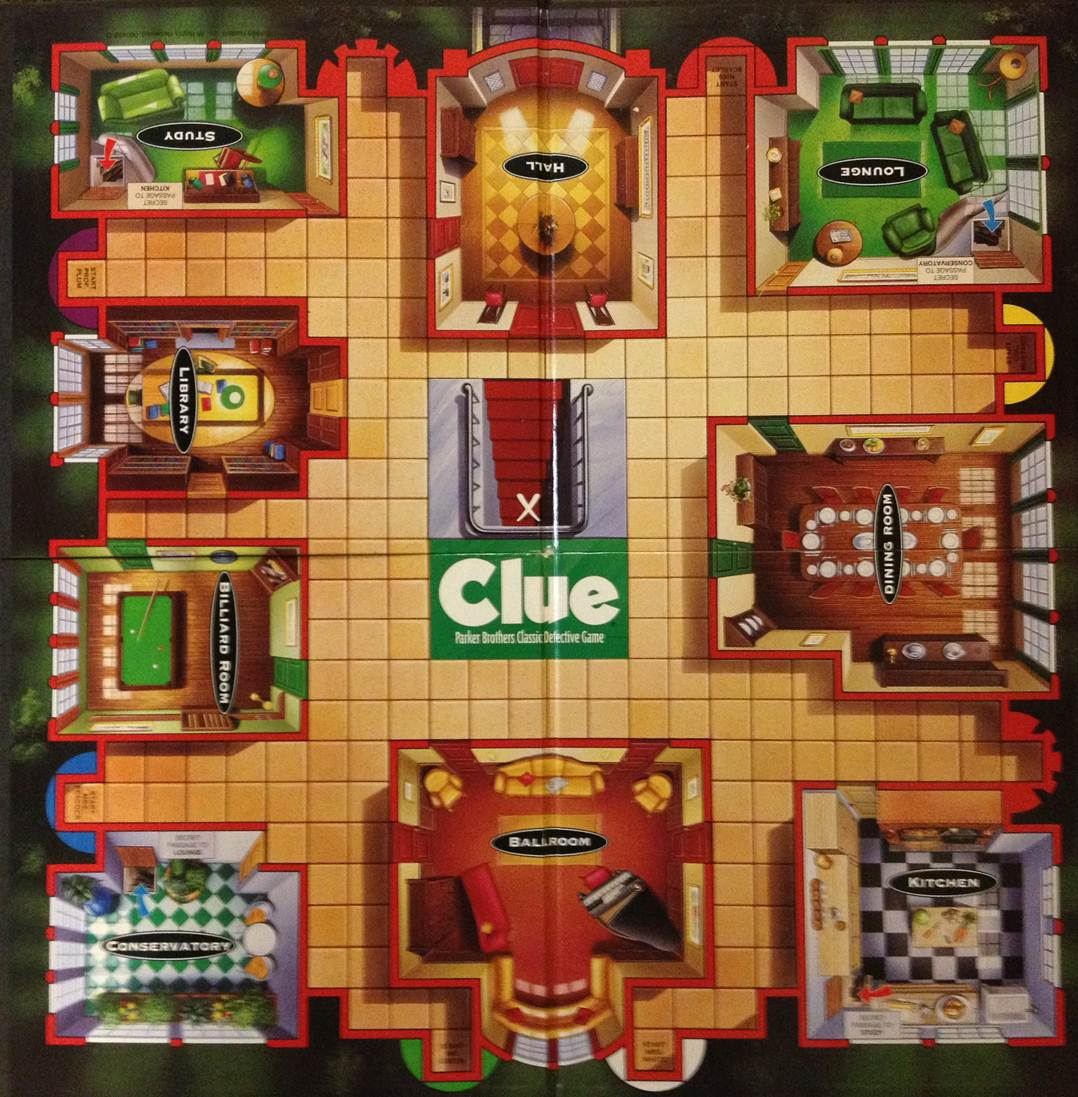
\includegraphics[height=0.7\textheight]{images/clue-board.jpg}
		\label{fig:game}
	\end{figure}
\end{frame}


\begin{frame}{Examples of Cards}
	\begin{figure}[h]
		\centering
		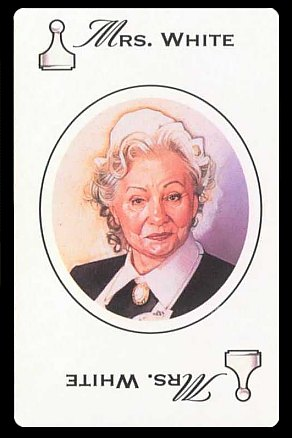
\includegraphics[width=0.3\textwidth]{images/cluewhite.jpg}
		\hfill
		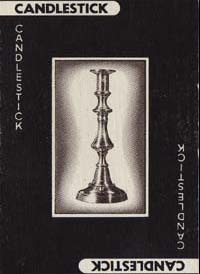
\includegraphics[width=0.3\textwidth]{images/CandleStick.jpg}
		\hfill
		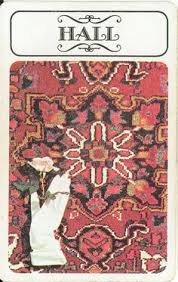
\includegraphics[width=0.3\textwidth]{images/hall.jpg}
		\label{fig:game}
	\end{figure}
\end{frame}

\begin{frame}{Our Project}
	Implementing a simplified version of the reasoning in Cluedo
\end{frame}